
\chapter{Finite Element Method for the Boussinesq modified equations}
\label{eulerian_bsq}


In this chapter, a FEM approximation for the Boussinesq modified equations is presented. Having a numerical approximation for the Boussinesq modified equations is mandatory when waves are studied on a two dimensional scenario and a complex bathymetry is considered.

Several numerical models appeared in the bibliography to solve the Boussinesq equations, under the possible variations for considering the dispersive terms. Abbot pioneered the FD schemes in \cite{abbott1978,abbott1979} applied to the original Boussinesq model. Later, Wei and Kirby solved the modified equations presented by Nwogu \cite{nwogu1993} using a FD scheme in \cite{wei1995}. The main advantage of the FD is the ease of treatment higher differences, even though the main difficulty consists on representing complex domains. Smallman was a pioneer applying the FD to harbours \cite{smallman1989}.

A decade later, some FEM were developed to solve Boussinesq equations. In that case, some special treatment needs to be applied to the high order derivatives. Langtangen \cite{langtangen1998} used quadratic triangles while most of the authors use aan intermediate variable. Li and Liu \cite{li1999} used bilinear quadrilaterals and used a projection to approximate the gradient. Walkley \cite{walkley2002} and Woo \cite{woo2004a,woo2004b} used a projection to interpolate the second order derivatives filed. Surprisingly, the authors reported high frequency oscillations and proposed ad-hoc solutions, but until Codina \cite{codina2008,codina2008b} none of them associated the oscillations to the incompatibility of interpolation.

The method has been solved using DG \cite{eskilsson2002} and FV \cite{bradford2002,stansby2003}. As reported by Stansby \cite{stansby2003}, since the FV is non-oscillatory, needs special techniques to accurately approximate the oscillatory behavior of the Boussinesq equations.

This chapter includes the developments presented in chapter \ref{eulerian_sw} and presents the new techniques associated to the oscillatory and dispersive problem. 
Som examples are included in order to test the accuracy and to show the capabilities of the presented algorithms.
Finally, the chapter is closed with the concluding remarks.



\section{Stabilized formulation for the Boussinesq modified equations}



As stated in section \ref{equations}, the Boussinesq equations and the Saint Venant equations are of the same family. Apart from the choice of different primary variables, the main difference consists on the inclusion of the dispersive terms. However, part of the structure of the equations remains unmodified.

The weak principle, the linear stabilization and the spatial discretization presented in section \ref{eulerian_sw} will be directly applied for the Boussinesq modified equations. The main differences arise from the dispersion terms.
First of all, the dispersion terms include spatial derivatives of order higher than two. Thus, special techniques for considering the third order derivatives will be included in the FEM procedure.

Secondly, the time discretization will be modified using a semi-implicit fourth-order scheme. The new time scheme allows to deal with the oscillatory behavior of the Boussinesq equations.
Additionally, the matrix structure will suffer some modifications related to the high order derivatives and the time integration scheme.

Regarding the shock capturing, usually it is not needed since the dispersion effect prevents from breaking and the formation of steep gradients. However, in the vicinity of the shoreline or very shallow domains, the amplitude dispersion effect could dominate over the frequency dispersion, making very recommended the inclusion of a shock capturing technique. Furthermore, if the shoreline is included, the shock capturing is required, since it provides stabilization for the moving front.

On another note, a section regarding the numerical treatment of absorbing boundary conditions is included. The inclusion of the frequency dispersion and the need of shortening the computational domain, lead to the open boundary conditions. On an open boundary conditions, waves can exit the computational domain and reflections must be avoided. The numerical approximation for the open boundary conditions are called absorbing boundary conditions.



% The Boussinesq modified equations need to be stabilized. In this section the linear stabilization presented in \ref{sec:fic_fem_stabilization} will be applied. Since the Boussinesq equations are intended to solve oscillatory problems, the shock capturing is not relevant. However, an additional technique must be introduced in order to deal with the higher order derivatives.

% In this section, the boundary conditions considered by the numerical model will be introduced. Then, the numerical procedure is explained. Here, the introduction of a gradient recovery is presented. After presenting the formulation for solving the equations, a numerical procedure for the absorbing boundary conditions will be proposed. Finally, some examples are added.





\subsection{Weak formulation and linear stabilization}


The Boussinesq equations are solved using the FEM. The background of chapter \ref{eulerian_sw} allows to interpolate the space domain with a Galerkin discretization of linear triangles or bilinear quadrilaterals. A finite difference scheme with constant time step is used to integrate the equations in time.

The variational form of the Boussinesq modified equations (\ref{bsq_eq}) presented in section \ref{equations_bsq} read
\begin{subequations} \label{bsq_eq_variational}
    \begin{equation}
        \int_\Omega\left(
        U\pder{\mathbf{u}_\beta}{t} + U\nabla \eta + U(\mathbf{u}_\beta \cdot \nabla) \mathbf{u}_\beta + U\mathbf{J}_u
        \right)d\Omega = \mathbf{0}
    \end{equation}
    \begin{equation}
        \int_\Omega\left(
        E\pder{\eta}{t} + E\nabla \cdot \left((H+\eta)\mathbf{u}_\beta\right) + E\nabla \cdot \mathbf{J}_\eta 
        \right)d\Omega = 0
    \end{equation}
\end{subequations}
where the auxiliary fields $\mathbf{J}_\eta$ and $\mathbf{J}_u$ are defined in (\ref{bsq_eq_auxiliary_J}) and involve second order derivatives of $\mathbf{u}_\beta$ and $\partial\mathbf{u}_\beta/\partial t$. E and V are the corresponding test functions for $\eta$ and $\mathbf{u}_\beta$.

In spite of the staggered formulation for the mass and momentum conservation, it is still a mixed wave formulation and the linear stabilization obtained by the FIC procedure will be applied. The additional term associated to the FIC residual could be projected onto a more general linearization matrix, including also the effects of the dispersive terms. However, the dispersive terms include different derivatives order. Since the current FIC stabilization only consider first order derivatives, the new residual term will be projected onto the fluxes matrices $\mathbf{A}_i$:
\begin{equation}
    \mathbf{A}_1 = \left[\begin{array}{ccc}
        u_{\beta1} &  0         &  g      \\
         0         & u_{\beta2} &  0      \\
         H+\eta    &  0         & u_{\beta1}
    \end{array}\right] \quad , \quad
    \mathbf{A}_2 = \left[\begin{array}{ccc}
        u_{\beta1} &  0         &  0      \\
         0         & u_{\beta2} &  g      \\
         0         & H+\eta     & u_{\beta2}
    \end{array}\right]
\end{equation}
where each term is obtained by linearization of the Boussinesq modified equations. The derivation of the full variational stabilized formulation is straightforward and for the sake of simplicity it is not shown.

% Some numerical difficulties such as the third order differential operator and the time integration accuracy are addressed in \cite{walkley2002,woo2004a,wei1995}.
% As stated by Codina in \cite{codina2008,codina2008b} the problem (\ref{bsq_eq}) is an hyperbolic wave in mixed form and there is an incompatibility condition (see \cite{BrezziFortin}) because the same interpolation is used for both variables, the velocity $\mathbf{u}_\beta$ and the wave amplitude $\eta$.
% Here the equations are stabilized using FIC extending the work done in \cite{maso2022}.



\subsection{High order derivatives and dispersive fields}

Following \cite{walkley2002}, the third order spatial derivatives are modelled using $\mathbf{J}_\eta$ as an intermediate variable. There are several ways of computing the intermediate field $\mathbf{J}_\eta$. The first possibility is to compute it in a monolithic way, adding $\mathbf{J}_\eta$ to the degrees of freedom.

A more interesting option is to compute it in a staggered way using a projection. In that case, the number of degrees of freedom is not increased and thus the time consuming performance of the scheme is unaltered. 

finally, the projection for the auxiliary field $\mathbf{J}_\eta$ can be replaced by a gradient recovery technique. In that section this option is analyzed, since the gradient recovery provides more regularity, at the same time, it is very efficient.

The gradient recovery technique was initially proposed by Zienkiewicz and Zhu in \cite{zienkiewicz1992}. Later, Zhang and Naga proposed some improvements for the super convergent gradient recovery in \cite{zhang2005} at boundaries. Finally, some improvements have been proposed in \cite{wu2007,ahmed2021} for adaptive meshes, but the last improvements are not going to be considered in this research. The basis of the gradient recovery consists on fitting a $k+1$ polynomial degree where the finite elements space is of degree $k$.


\subsubsection{Algorithm}

The main idea of the gradient recovery is to introduce an operator $G_h : S_h \rightarrow S_h^{n_d}$, where $S_h$ is a polynomial finite element space of degree $k$ over a triangulation $T_h$ and $n_d$ is the space dimension. After determining the values of $G_h$ at all nodes, given a solution $u_h$ , $G_h u_h \in \S_h^{n_d}$ is obtained on the whole domain.
The triangulation can be replaced by a quadrilateral discretization. In both cases, only vertices nodes are considered, nor edge or internal nodes.

For a vertex $\mathbf{x}_i$ and being $l_i^e$ the size of the largest edge attached to $\mathbf{x}_i$, a ball is defined around it:
\begin{equation}
    B_{l_i^e}(\mathbf{x}_i) = \{ \mathbf{x} \in T_h : \vert \mathbf{x} - \mathbf{x}_i \vert \leq l_i^e \}
\end{equation}
and all the vertices inside the ball are selected. If the number of nodes $n_n$ inside the ball $B_{l_i^e}(\mathbf{x}_i)$ is less than $m = (k+n_d) (k+n_d+1) / 2$, then the ball is extended to two times the edge length, $B_{2l_i^e}$. This process of increasing the radius is repeated until there are enough nodes in the ball. The nodes inside a ball are denoted as $\mathbf{x}_{ij}$ and the polynomial $p_{k+1}$ is fitted using local coordinates with $\mathbf{x}_i$ at the origin and the scaling parameter $l=l_i^e$,
\begin{equation}
    p_{k+1} = \mathbf{P}^T \mathbf{a} = \hat{\mathbf{P}}^T \hat{\mathbf{a}}
\end{equation}
where
\begin{subequations}
\begin{equation*}
         \mathbf{P}^T  = (1,x,y,x^2,...,x^{k+1},x^ky,...,y^{k+1}), \quad
    \hat{\mathbf{P}}^T = (1,\xi,\eta,\xi^2,...,\xi^{k+1},\xi^k\eta,...,\eta^{k+1})
\end{equation*}
\begin{equation*}
         \mathbf{a}^T  = (a_1,a_2,...,a_m), \quad
    \hat{\mathbf{a}}^T = (a_1,la_2,...,l^{k+1}a_m),
\end{equation*}
\end{subequations}
And the coefficient vector $\mathbf{a}$ is determined by the linear system
\begin{equation} \label{superconvergent_polynomial}
    A^T A \hat{\mathbf{a}} = A^T \mathbf{b}_h
\end{equation}
where $\mathbf{b}_h^T = (u_h(\mathbf{x}_{i1}), u_h(\mathbf{x}_{i2}), ... , u_h(\mathbf{x}_{in_n}))$ and
\begin{equation*}
A = \left(\begin{matrix}
    1 & \xi_1 & \eta_1 & ... & \eta_1^{k+1} \\
    1 & \xi_2 & \eta_2 & ... & \eta_2^{k+1} \\
    \vdots & \vdots & \vdots & \ddots & \vdots \\
    1 & \xi_{n_n} & \eta_{n_n} & ... & \eta_{n_n}^{k+1} \\
\end{matrix}\right)
\end{equation*}
A condition for (\ref{superconvergent_polynomial}) having solution is that $Rank(A) = m$, which is practically always satisfied when $n_n > m$ and the mesh has a reasonable quality. Finally, it is possible to define the gradient at the point $\mathbf{x}_i$ as
\begin{equation}
    G_h u_h (\mathbf{x}_i) = \nabla p_{k+1} (0,0,\mathbf{x}_i)
\end{equation}

Similarly, the gradient of a divergence can be obtained when the polynomial is applied to a vector field. This procedure can be applied up to derivatives of order $k+1$, which for linear elements are second-order derivatives. Finally, the gradient of the divergence reads
\begin{equation}
    L_h u_h (\mathbf{x}_i) = \nabla \nabla \cdot p_{k+1} (0,0,\mathbf{x}_i)
\end{equation}

Since the values of the nodal unknowns $u_h$ are not known a priory, the vector of coefficients $\mathbf{a}$ will be expressed as a linear combination of $u_h(\mathbf{x}_{ij})$. Depending on which derivatives of $\mathbf{P}$ are seek, the linear combination will be some selected rows of $(A^T A)^{-1}A^T$.




\subsection{Time discretization}

Finally, the problem (\ref{bsq_eq}) is expressed in matrix form as
\begin{equation} \label{sw_system_matrix}
    (M + K) \dot{x} = F(x,y)
\end{equation} 
where $x$ is the vector of nodal unknowns, $y$ is the vector of nodal values corresponding to $\mathbf{J}_\eta$, $M$ is a mass matrix, $K$ correspond to the second derivatives associated to $\mathbf{J}_{\mathbf{u}}$, and $F$ is a non-linear vector which is a function of $\mathbf{u}_\beta$ and its spatial derivatives.



The commonly used fourth order Adams-Moulton scheme is employed for the time integration of (\ref{sw_system_matrix}), see \cite{wei1995,woo2004a,codina2008b} as an example.
To obtain a solution at the time step $t^{n+1}$, the fixed point iterative method is employed to deal with the non-linearity of the system. Given a guess $x^{n+1,i-1}$ for $x^{n+1,i}$ at iteration $i$, the increment $\delta x^i$ is computed from
\begin{multline}
    24 (M + K) \delta x^i = 
    24 (M + K) (x^n - x^{n+1,i-1}) \\
     + \delta t (9F^{n+1} + 19F^n - 5F^{n-1} + F^{n-2}) + O(\delta t^4)
    \label{adams-moulton}
\end{multline}
The time integration is closed using the explicit third order Adams-Bashforth scheme to predict the initial guess $x^{n+1,0}$ for the non-linear iterations
\begin{multline}
    12 (M + K) x^{n+1,0} = 
    12 (M + K) x^n \\
     + \delta t (23F^n - 16F^{n-1} + 5F^{n-2}) + O(\delta t^3)
    \label{adams-bashforth}
\end{multline}

The system of (\ref{adams-moulton}) and (\ref{adams-bashforth}) is solved using a direct solver. Given the problem is small, this is not expensive.
Convergence is achieved when $\delta x^i$ is sufficiently small. Then, the solution $x^{n+1}$ is set as $x^{n+1,i}$.





\subsection{Absorbing boundary conditions}
\label{eulerian_bsq_absorbing}


Frequently, the need to shorten the numerical domain arises. This can be achieved by the imposition of open boundaries, also known as radiant boundaries. The open boundaries allow the exit of the waves as well as the consistency of the system of equations in order to ensure the existence and uniqueness of the solution. Additionally, the numerical tool for the boundary has to be compatible with the numerical approach for the inner domain.

Generally, the radiant boundary condition denotes the analytical formulation for open boundaries and the term absorbing boundary is related to the numerical approximation of the radiation condition \cite{navon2004}. An equilibrium between the precision offered by the radiant boundary and the numerical cost required by the absorbing boundary is seek.
From one side, the boundary conditions must define a well posed problem and the spurious oscillations in the open boundary shall be as small as possible. From the other side, the computational cost of the boundary conditions should be small compared to the computational cost of the inner domain.

Considering the unidirectional wave propagation and being $\eta$ the free surface elevation, a wave function will verify a radiant boundary condition where
\begin{equation} \label{radiation_condition}
    \pder{\eta}{t} + c \cos(\theta)\pder{\eta}{x} = 0
\end{equation}
where $\theta$ is tha incidence angle of the wave with respect to the boundary.

Some authors proposed local approximations highly diffusives \cite{engquist1977}. Latter, Bayliss explored the radiation boundary conditions for the Helmholtz equations in \cite{bayliss1982}.
Similarly, Collino \cite{collino1993} extended the formulation using higher order of derivatives than \ref{radiation_condition}. However, the generalization for the Euler equations -analogously the SW equations- in 2 or 3D is not trivial, since the incidence angle $\theta$ is not known \emph{a priori} and because of the dispersive behavior of the equations \cite{wei1995}.

The dispersive behavior is associated to the fact that there is not an unique celerity characterizing the system: in the case of the SW or the Boussinesq equations there are three waves superposed propagating at different speeds. For example, in section \ref{sec:sw_fc} a decomposition in characteristics was presented through diagonalization of the tangent matrices $\mathbf{A}_i$.
\begin{equation}
    \pder{\bm\Phi_j}{t} + \bm\Lambda_i \pder{\bm\Phi_j}{x_i} = 0
\end{equation}
in that minimal wave equation $\bm\Lambda$ is a diagonal matrix such that $\bm A_i = \bm T_i \bm\Lambda_i \bm T_i^{-1}$.
This problem can be understood a the superposition of three waves, each one of them propagating at speed $u-c$, $u$ y $u+c$, namely the eigenvalues $\lambda_i$. The sign of $\lambda_i$ determines if the wave is incoming or outgoing and the regime of the problem: subcritical or supercritical.

Besides having to impose the radiant boundary condition for the three waves, this approximation is limited, since in 2 or 3D does not exist a genuine characteristic-based formulation. A more detailed development can be found in \cite{lie2001}.

Most of the proposals to approximate the open boundaries consist on relaxing the condition \ref{radiation_condition}  adding a dissipation term $K$ and extending the domain a distance $d$, losing the local definition. See \cite{israeli1981,navon2004,carmigniani2018} as an example. Then, the radiation condition is rewritten as
\begin{equation} \label{radiation_absorbing_condition}
    \pder{\eta}{t} + c \cos(\theta)\pder{\eta}{x} = -K\eta
\end{equation}
This approximation can be used in combination with local absorbing boundary conditions \cite{wei1995}.

Another of the explored possibilities is the Perfectly Matched Layer (PML) \cite{berenger1994}, widely used in the literature. It presents the inconvenient of special treatment of corners.
Later, this methodology wa used in combination with the high order absorbing boundaries, leading to the Double Absorbing Boundary (DAB), proposed by Hagstrom and Rabinovich in \cite{hagstrom2014,rabinovich2015}. This technology places two parallel boundaries separated by a short distance. Its advantage is that they do not need to incorporate the derivatives in the normal direction neither to apply any special treatment to the corners.

Finally, and given to the simplicity of the formulation, there is the possibility of including only a sponge layer. It can be found in the formulations of Israeli and Carmigniani in \cite{israeli1981,carmigniani2018}. A Newtonian dissipative term analogous to the bottom friction $S_f$ is added as
\begin{equation}
    S_a = -\gamma(\mathbf{x}) \mathbf{u}
\end{equation}
The dissipative term $\gamma$ varies from 0 at a given distance to the discrete boundary to the maximum value $\gamma_{max}$ at the discrete boundary. This variation follows an exponential law \cite{peric2018} of order $n$. The parameters of the sponge layer $d_0$ and the maximum value $\gamma_{max}$ need to be specified for each case, in terms of the wavelength.
A possible expression for $\gamma$ is
\begin{equation} \label{exponential_sponge_layer}
    \gamma(\mathbf{x}) = \gamma_{\max} \mathcal{H}(d_0 - d(\mathbf{x})) \frac{e^{\left(\frac{d_0 - d(\mathbf{x})}{d_0}\right)^n} - 1}{e - 1}
\end{equation}
where $\mathcal{H}$ is the Heaviside function, $d$ is the distance from a point to the computational boundary.

In Fig. \ref{absorbing_boundary} the propagation of a train of regular waves is shown. Ate the left end of the domain, waves are generated. At the right end of the domain there is a sponge layer. Studies carried out by Carmigniani in \cite{carmigniani2018} show that some combinations of the maximum absorption, layer width and exponential degree can produce undesired reflections. For example, an excessive absorption can generate reflections at the beginning of the sponge layer.

An exponent $n=3$ for expression \ref{exponential_sponge_layer} is chosen, it considerably minimizes the reflection \cite{carmigniani2018}. A sensibility analysis of the parameters $d_0$ y $\gamma_{\max}$ should be done.
It is useful to express the maximum distance and absorption in terms of the wavelength and frequency. In practice, the width of the sponge layer is used to be $d_0 \approx 2\lambda$ and the absorption coefficient $\gamma \approx 0.5\omega$.

The reflected amplitude is monotonically decreasing as the sponge width increases. Nevertheless, the reflection exhibits a local minimum with respect to the absorption coefficient. This makes highly recommended to adjust the parameters of the sponge layer according to the  maximum wavelength.


\begin{figure}
    \centering
    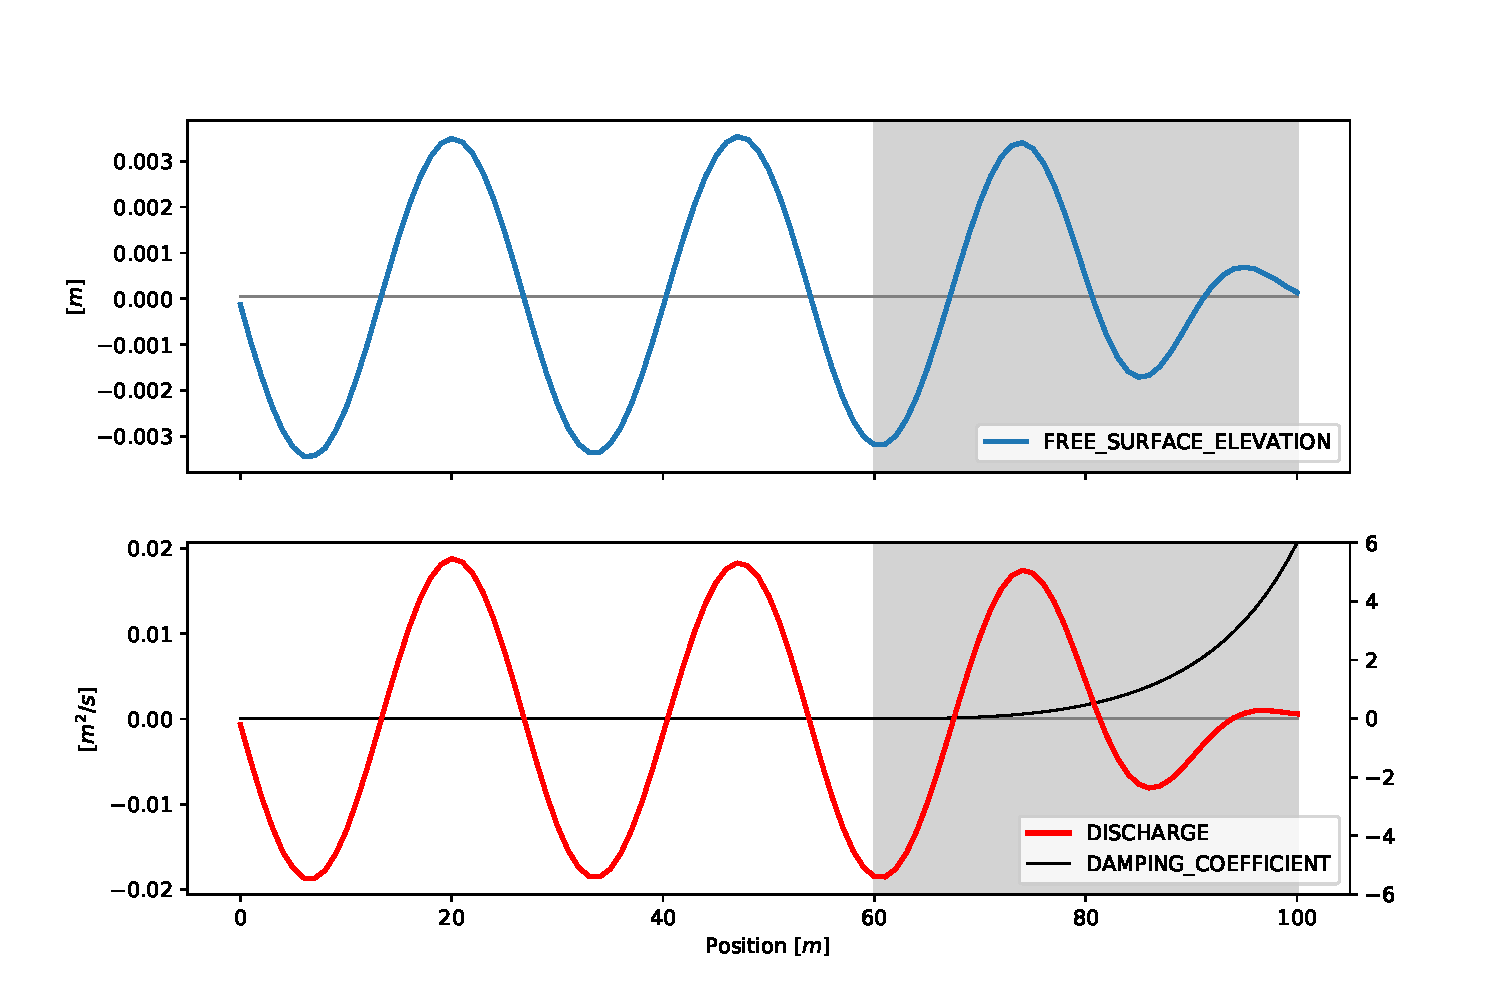
\includegraphics[width=.8\textwidth]{img/absorbing_boundary/absorbing_boundary.pdf}
    \caption{Propagation and absorption of a train of waves. The shadow region shows the width of the sponge layer.}
    \label{absorbing_boundary}
\end{figure}


\section{Examples}


\subsection{Solitary wave propagation}


\subsection{Absorbing boundary}



\section{Concluding remarks}


